\documentclass[12pt]{article}


\usepackage{graphicx} % This lets you include figures
\graphicspath{ {images/} }
\usepackage{hyperref} % This lets you make links to web locations

\usepackage{mathtools}
\usepackage{amssymb}
\interdisplaylinepenalty=2500

\usepackage{varioref}

\usepackage{dblfloatfix}
\usepackage{xcolor}
\usepackage{underscore}
\usepackage[T1]{fontenc}
%\usepackage{lmodern}

\usepackage[section]{placeins}
%\usepackage[subsection]{placeins}

\makeindex


\title{\textbf{\textsc{HELMpy} \\ User's Guide}}
\author{Tulio Molina \hspace{10mm} Juan Ortega}
\date{\today}

\begin{document}
\sloppy

\maketitle{}
\thispagestyle{empty}
\tableofcontents
\clearpage
\newpage


\section{Introduction}

\textsc{HELMpy} \cite{HELMpy} is an open source package of power flow solvers developed on Python 3 \cite{python}. This package contains the Holomorphic Embedding Load-flow Method (HELM) \cite{trias2012holomorphic} and the Newton-Raphson (NR) algorithm. The intention of \textsc{HELMpy} is to support research, especially on the HELM, and to contribute with the development of open source code related to this subject. The developed code is properly commented and organized so it would be easy to understand and modify. This package was developed by Tulio Molina and Juan José Ortega as a part of their thesis research to obtain the degree of Electrical Engineer at Universidad de los Andes (ULA) in Mérida, Venezuela. 

\subsection{License and Terms of Use}
The code is distributed under the GNU Affero General Public License v3.0  or later \cite{GNUAGPLv3} (AGPL-3.0-or-later). The full text of the license can be found in the \texttt{LICENSE.txt} file.

\section{Power Flow}
The solution to the power flow problem consists in calculating the voltage at each bus of a power system under steady-state and balanced conditions, and this is carried out by solving a set of nonlinear equations that arises with the well known power balance equations. It is important to remark that the classic single slack bus model for the power flow problem uses a unique bus to account for system losses, on the orther hand, Distributed Slack Bus (DSB) models state that active power losses of the system can be distributed among system's generators in order to obtain a more realistic modeling of power systems. DSB models based on the allocation of participation factors to each generator are widely implemented on the literature, and several approaches have been formulated to calculate these participation factors based on different criteria. In \cite{meisel1993system}, participation factors are calculated depending on each generator's active power output. 

Power systems modeling and algorithms implemented in \textsc{HELMpy} for solving the power flow problem are explained below.

\subsection{Modeling}
The power flow solvers included in \textsc{HELMpy} implement the standard \boldmath{$\pi$} branch model, which models transmission lines, phase-shifting transformers and off-nominal
tap transformers. Shunt admittances for modeling capacitors or reactors banks in parallel to buses are also considered. Besides, reactive power limits at generators are as well taken into account, in exception for the slack's bus generator.

\subsection{Algorithms}

\subsubsection{HELM}
The HELM, firstly proposed by Antonio Trias \cite{trias2012holomorphic}, is a power flow method based on the study of complex analysis. The method is fully implemented in \textsc{HELMpy}. The theory, fundamentals and practical implementations used as guide to implement this method are described and presented in \cite{subramanian2014application}, \cite{rao2016holomorphic} and \cite{trias2015fundamentals}. The method is developed considering two different models for PV buses, as the ones described in \cite{subramanian2014application}.
 
HELM, seen solely as a numeric method, consists in recursively solving a linear matrix equation of the form $A\,x=B$ and, after each time this system is solved, performing analytic continuation on a group of power series that represent voltages at buses; this process continues until convergence is reached or divergence is detected. The matrix $A$ remains constant, so it should be factorized. The vector $B$ is computed before each time the system is to be solved. As a result, vector $x$ contains a new coefficient of each voltage power series. 

\begin{figure}[!h]
	\centering
	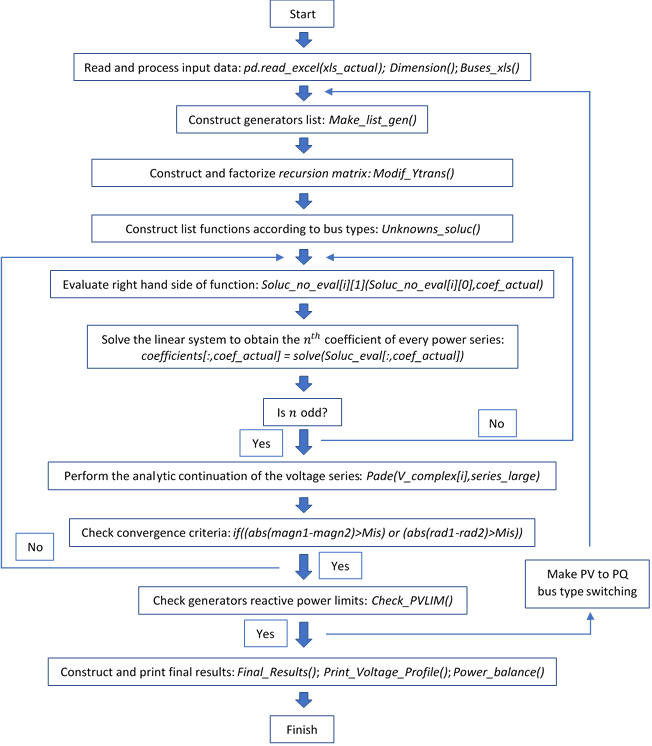
\includegraphics[width=\textwidth]{helmflowchart}
	\caption{HELM flow chart}
	\label{helmflowchart}
\end{figure}

Figure \ref{helmflowchart} \vpageref{helmflowchart} contains the flowchart that exposes the procedure of the method (solely as a numeric method) and shows the respective and relevant functions and code lines that execute those steps.

\subsubsection{Newton-Raphson}
The extensible used Newton-Raphson algorithm to solve the power flow problem is implemented using complex numbers in rectangular form for calculations and unknown variables are represented in polar form.

\begin{figure}[!h]
	\centering
	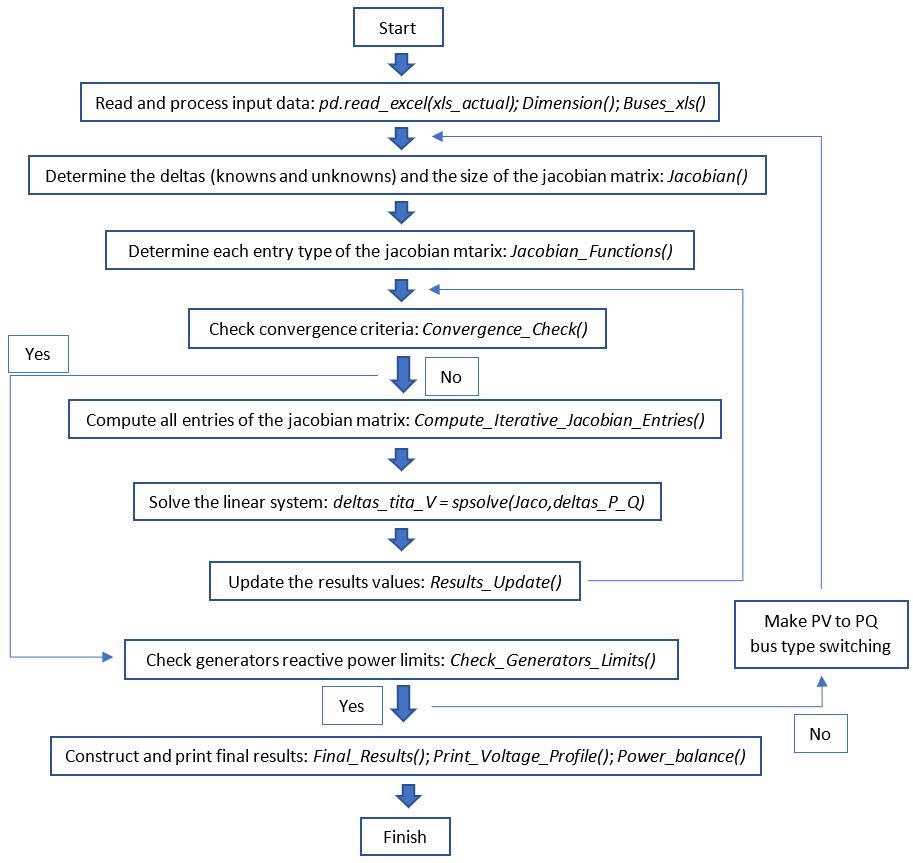
\includegraphics[width=\textwidth]{nrflowchart}
	\caption{Newton-Raphson flow chart}
	\label{nrflowchart}
\end{figure}

Figure \ref{nrflowchart} \vpageref{nrflowchart} contains the flowchart that exposes the procedure of the method (solely as a numeric method) and shows the respective and relevant functions and code lines that execute those steps.

\subsubsection{Distributed Slack Bus Model}
A DSB model for the power flow formulation based on participation factors described in \cite{meisel1993system} is developed in \textsc{HELMpy} for both HELM and NR methods. The DSB model for NR is obtained from \cite{tong2005network} and implemented to balanced systems. Furthermore, considering PV bus models defined in \cite{subramanian2014application}, four implementations of such DSB model for HELM are developed and denominated as: M1 PV1, M1 PV2, M2 PV1 and M2 PV2, according to the selected model for describing the slack and PV buses. This combinations depends on the chosen arguments when executing the helm function.

\subsubsection{Convergence criteria}
Considering a maximum mismatch error, the managed convergence criteria for the NR implementation is based on checking active and reactive power mismatch error at each bus, according to the bus type. On the other hand, the managed convergence criteria for implementations based on the HELM consists in checking whether the difference between the magnitudes and phase angles of two consecutive voltages (obtained through analytic continuation of power series) at each bus is less than the mismatch error.

\section{How to use \textsc{HELMpy}}

\subsection{Software requirements}
\textsc{HELMpy} is written in Python version 3.6.0, therefore, this or newer versions of the aforementioned programming language along with the following libraries must be installed in order to use this power flow solver package:
\begin{itemize}
	\item \texttt{Numpy} \cite{numpy}
	\item \texttt{Scipy} \cite{scipy}
	\item \texttt{Pandas} \cite{pandas}
\end{itemize}

No installation process other than copying the files of \textsc{HELMpy} folder to the directory where \textsc{HELMpy} is going to be used is needed.

\subsection{Input case}
For purposes of portability and simplicity \textsc{HELMpy} receives as input case (grid or system) a \texttt{.xlsx} file which contains all the needed data to solve a power flow problem.

\subsubsection{Obtaining a case from \textsc{Matpower}}
The format of the input \texttt{.xlsx} file has been designed from the format of \textsc{Matpower} \cite{matpower} cases. Therefore, the script \texttt{Obtain_case_MATPOWER.m}, which is a template for obtaining the \textsc{HELMpy} input data of the desired grid stored in \textsc{Matpower}, is included in the \textsc{HELMpy} folder. By means of this \texttt{.m} script, case9, case118, case1354pegase and case2869pegase stored in \textsc{Matpower} have been processed and their respective \texttt{.xlsx} files (of the same name) are also included in the data/cases folder of the \textsc{HELMpy} repository.

\subsubsection{Creating a case:}
The \texttt{.xlsx} file for the input case can be created by the user. Such file must contain three sheets, without header, named as follows: \textsl{Buses}, \textsl{Generator} and \textsl{Branches}. According to the sheet, the data that must be stored in each column is presented below: \\

\begin{itemize}
	\item \textsl{Buses}, each row stands for a bus of the grid:
	\begin{itemize}
		\item Column A: Bus number (positive integer).
		\item Column B: Type of buses. 1 for PQ, 2 for PV, 3 for slack.
		\item Column C: Active power demand (MW).
		\item Column D: Reactive power demand (MVAr).
		\item Column E: Shunt conductance (MW demanded at V = 1.0 p.u.).
		\item Column F: Shunt susceptance (MVAr injected at V = 1.0 p.u.).
	\end{itemize}

	\item \textsl{Generators}, each row stands for a generator of the grid:
	\begin{itemize}
		\item Column A: Bus number (positive integer).
		\item Column B: Active power output (MW).
		\item Column D: Maximum reactive power output (MVAr).
		\item Column E: Minimum reactive power output (MVAr).
		\item Column F: Voltage magnitude set point (p.u.).
	\end{itemize}

	\item \textsl{Branches}, each row stands for a branch of the grid:
	\begin{itemize}
		\item Column A: “From” bus number.
		\item Column B: “To” bus number.
		\item Column C: Resistance (p.u.).
		\item Column D: Reactance (p.u.).
		\item Column E: Total line charging susceptance (p.u.).
		\item Column I: Transformer off nominal turns ratio (taps at “from" bus, impedance at “to" bus).
		\item Column J: Transformer phase shift angle (degrees), positive for delay.
	\end{itemize}
\end{itemize}

The remaining columns are not used. The input file must be in the directory where \textsc{HELMpy} is going to be used.

\subsection{Functions}
As it has been said, \textsc{HELMpy} is able to solve the power flow problem by means of the NR method or by the HELM considering whether PV bus model I or II is used, and also applying the DSB models. These methods are developed to be used as the following functions:
\begin{itemize}
	\item \texttt{nr(GridName, Print_Details=False, Mismatch=1e-4,\\ Results_FileName="", Scale=1, MaxIterations=15,\\ Enforce_Qlimits=True)}
	%
	\item \texttt{nr_ds(GridName, Print_Details=False, Mismatch=1e-4,\\ Results_FileName="", Scale=1, MaxIterations=15,\\ Enforce_Qlimits=True, DSB_model=True)}
	%
	\item \texttt{helm(case, detailed_run_print=False, mismatch=1e-4, scale=1, max_coefficients=100, enforce_Q_limits=True, results_file_name=None, save_results=False, pv_bus_model=2, DSB_model=False, DSB_model_method=None)}
	%
\end{itemize}

Where the parameters of the NR functions are explained below:
%
\begin{itemize}
	\item[--] \texttt{GridName}: String of characters type. This parameter receives the name of the input grid. The \texttt{.xlsx} extension must be included in the string of characters. 
	\item[--] \texttt{Print_Details}: Boolean type. If \texttt{True}, the function prints details of the running power flow problem and the results of it on the Python console, if \texttt{False}, it only prints whether convergence was reached or not. This parameter is set as \texttt{False} by default.
	\item[--] \texttt{Mismatch}: Float type. It defines the value of the maximum mismatch error. This parameter is set at \texttt{1e-4} by default.
	\item[--] \texttt{Results_FileName}: String of characters type. The received string of characters is used for naming the \texttt{.txt} and \texttt{.xlsx} output files along with other information (used function, \texttt{Scale} and \texttt{Mismatch}). The name will be the same as the input case file if this parameter is an empty string of characters. It is set as an empty string of characters by default.
	\item[--] \texttt{Scale}: Float or integer type. It receives the scaling factor which multiplies active and reactive power load and active power generation of the grid (loadability scaling factor). This parameter is set at 1 by default.
	\item[--] \texttt{MaxIterations}: Integer type. It defines the maximum number of iterations allowed for reaching convergence. The number of iterations is restarted if convergence is reached but reactive power limits are violated. It is set at 15 by default.
	\item[--] \texttt{Enforce_Qlimits}: Boolean type. If \texttt{True}, reactive power generation limits are checked at each PV bus after convergence is reached, if \texttt{False}, limits are not checked. It is set as \texttt{True} by default.
\end{itemize}

And the parameters of the helm function are explained below:
%
\begin{itemize}
	\item[--] \texttt{case}: Case data object, contains the grid data.
	\item[--] \texttt{detailed_run_print}: Boolean type. If \texttt{True}, the function prints details of the running power flow problem and the results of it on the Python console, if \texttt{False}, it only prints whether convergence was reached or not. This parameter is set as \texttt{False} by default.
	\item[--] \texttt{mismatch}: Float type. It defines the value of the maximum mismatch error. This parameter is set at \texttt{1e-4} by default.
	\item[--] \texttt{scale}: Float or integer type. It receives the scaling factor which multiplies active and reactive power load and active power generation of the grid (loadability scaling factor). This parameter is set at 1 by default.
	\item[--] \texttt{max_coefficients:} Integer type. It defines the maximum number of coefficients to be computed by the algorithm for reaching convergence. The number of coefficients is restarted if convergence is reached but reactive power limits are violated. It is set at 100 by default.
	\item[--] \texttt{enforce_Q_limits}: Boolean type. If \texttt{True}, reactive power generation limits are checked at each PV bus after convergence is reached, if \texttt{False}, limits are not checked. It is set as \texttt{True} by default.
	\item[--] \texttt{results_file_name}: String of characters type. The received string of characters is used for naming the \texttt{.txt} and \texttt{.xlsx} output files along with other information (used function, \texttt{Scale} and \texttt{Mismatch}). The name will be the same as the input case file if this parameter is an empty string of characters. It is set as an empty string of characters by default.
	\item[--] \texttt{save_results}: Boolean type. If \texttt{True}, a results file is generated and save, if \texttt{False}, ir is not. It is set as \texttt{False} by default.
	\item[--] \texttt{pv_bus_model:} Integer type. Options available \{1,2\}. If \texttt{1}, the pv bus model 1 is used. If \texttt{2}, the pv bus model 2 is used. It is set as \texttt{2} by default.
	\item[--] \texttt{DSB_model:} Boolean type. If \texttt{True}, the DSB is used, if \texttt{False}, the slack bus is set to account for all losses representing in this way the classic bus model. It is set as \texttt{True} by default.
	\item[--] \texttt{DSB_model_method:} Integer type. Options available \{1,2\}. If \texttt{1}, the DSB model 1 is used. If \texttt{2}, the DSB model 2 is used. It is set as \texttt{None} by default. If the DSB_model is set to \texttt{True}, DSB_model_method is set to 2.
\end{itemize}


Each one of these functions returns the resultant voltage profile given in complex rectangular form.


\subsection{Output files}
In order to show and save the output of each program execution, two files are generated: a \texttt{.xlsx} file and a \texttt{.txt} file.

The resultant voltage profile, in complex and polar form, is presented in the \textit{Buses} sheet of the resultant \texttt{.xlsx} file. On the other hand, the power injection of buses through each branch of the grid is shown in the \textit{Branches} sheet of such file.

Information such as loadability scale factor, convergence time, mismatch error, number of coefficients or number of iterations (according to the used function), and also a power balance of the problem are shown in the output \texttt{.txt} file.

\subsection{Running \textsc{HELMpy}}
Each one of the aforementioned functions can be imported to the user’s Python script by declaring the command:
\newline \\
%
\hspace*{5mm} \texttt{import helmpy}\\

The \texttt{helmpy.py} script imports the \texttt{nr}, \texttt{nr_ds} and \texttt{helm} functions from the respective \texttt{.py} script where each one of them is defined. Therefore, for running \textsc{HELMpy} with a pre-defined input case named \texttt{Case.xlsx}, by means of these three functions, a typical Python script would look as follows: \\ \\
%
\hspace*{5mm} \texttt{import helmpy\\\\
\hspace*{5mm} voltage_profile_nr = helmpy.nr("Case.xlsx")\\
\hspace*{5mm} grid_data_file_path = '/path/of/case.xlsx'
\hspace*{5mm} voltage_profile_helm = helmpy.helm(case.case)\\}

Where the resulting voltage profile of each function is returned to its corresponding assigned variable.

\subsection{Comparing results}
The following \texttt{.py} scripts found on the test folder can be used to compare voltage profile results obtained from \textsc{HELMpy} and \textsc{Matpower}:
\begin{itemize}
	\item \texttt{Compare_Voltages.py}: It compares two voltage profiles obtained from \textsc{HELMpy}. The absolute value of the highest magnitude and phase angle differences between both voltage profiles are printed on the Python console. If the \texttt{print_all} variable is set as \texttt{True}, the absolute value of the magnitude and phase angle differences at each bus are also going to be printed.
	\item \texttt{Compare_Several_Voltages.py}: It compares one voltage profile (base profile) with a list of voltage profiles obtained from \textsc{HELMpy}. The absolute value of the highest magnitude and phase angle differences between the base profile and the rest of profiles are printed on the Python console, respectively. If the \texttt{print_all} variable is set as \texttt{True}, the absolute value of the magnitude and phase angle differences at each bus are also going to be printed.
	\item \texttt{Compare_with_MATPOWER.py}:  It compares two voltage profiles, one obtained from \textsc{HELMpy} and the other obtained from \textsc{Matpower}. The absolute value of the highest magnitude and phase angle differences between both voltage profiles are printed on the Python console. If the \texttt{print_all} variable is set as \texttt{True}, the absolute value of the magnitude and phase angle differences at each bus are also going to be printed.
\end{itemize}

There are \texttt{.xlsx} files of already computed results results in the data/results folder of the repository for reference and comparison.

\section{Miscellaneous}
In order to validate the results obtained from \textsc{HELMpy}, a comparison between these results and the ones obtained from \textsc{Matpower} can be made, for such, the \texttt{\mbox{Execute_MATPOWER.m}} script is included in the \textsc{HELMpy} folder. This script allows to run a power flow problem with \textsc{Matpower} by means of the NR method, where loadability scale factor of the case, tolerance and initial seed of voltages can be modified. The output of \texttt{Execute_MATPOWER.m} is a \texttt{.xlsx} file containing the resultant voltage profile, which can be used by the \texttt{\mbox{Compare_with_MATPOWER.py}} script.

The mentioned \texttt{.m} script has been used to execute case9, case118, case1354pegase and case2869pegase using a tolerance of \texttt{1e-8}. Their respective \texttt{.xlsx} output files are named ``\texttt{Results MATPOWER case9.xlsx}'', ``\texttt{Results MATPOWER case118.xlsx}'', ``\texttt{Results MATPOWER case1354pegase.xlsx}'' and ``\texttt{Results MATPOWER case2869pegase.xlsx}''. These files are included in the \texttt{HELMpy} folder.


% references section
\bibliographystyle{IEEEtran}
\nocite{*}
\bibliography{IEEEabrv,bibliografia}

\end{document}



%\colorbox{green}{\parbox{8.75cm}{ texto texto texto }}














